\chapter{多大语言模型系统中的涌现行为}\label{chap:emergent}

\begin{learningbox}
本章将介绍多个大语言模型智能体在{\em 未被分配角色}时如何行动，以研究开放式系统中的涌现行为。
具体而言，学完本章后，你将能够：
\begin{itemize}[leftmargin=*, nosep]
    \item 区分研究涌现行为的多智能体模拟与基于角色的交互，并解释为什么开放式环境需要不同的{\em 研究问题与评估}方法。
    \item 描述生成式智能体模拟的{\em 架构}，以及模拟基础设施如何从少量智能体扩展到数千个智能体。
    \item 解释全局层面的惯例、规范与元规范如何从局部层面的智能体自然语言交互中{\em 涌现}。
    \item 理解多智能体模拟如何在计算社会科学中用作{\em 科学工具}。
    \item 理解{\em 开放世界}基准环境对数据生成的重要性。
    \item 批判性地评估从人类语境引入的概念，如涌现、自组织与集体智能，其相关主张是否有效，并评估开放式多智能体系统带来的{\em 安全风险}。
\end{itemize}
\end{learningbox}

\section{什么是多智能体涌现行为？}\label{sec:interacting}
上一章研究的多大语言模型系统为每个智能体分配了角色，并通过协议引导交互。其研究问题关注智能体在指定结构内的行为，考察一组智能体能够在受控条件下多好地解决任务。本章则将智能体置于开放式环境中，研究问题也从\emph{在给定全局结构下，智能体如何行动、表现如何？}转向\emph{局部智能体的交互会涌现出什么全局结构？}

正如本书前文所述，智能体大语言模型（agentic LLM）在感知、记忆、推理、决策与适应性学习方面具有增强的能力，也能呈现不同的性格特征 \citep{gao2023s, gao2024large}。这些特点使它们适合在不预先分配角色的开放式多智能体模拟中交互，作为社会中人类行为的替代模型。由于大语言模型智能体使用自然语言交流，研究者能够阅读和解释模拟中的交互。这让研究者得以观察中间步骤，也使这类模拟与人类交互之间的可比性远高于经典框架中的模拟，回应了社会科学领域长期以来的研究兴趣。图~\ref{fig:abm}~和图~\ref{fig:struct}~展示了适用于此类模拟的大语言模型智能体的一般结构。

\begin{figure}
  \begin{center}
    \begin{tikzpicture}[x=1cm,y=1cm,>=Stealth,font=\small,
  req/.style={draw=blue!35!black,fill=blue!66!gray,text=white,rounded corners=2pt,
    minimum width=2.15cm,minimum height=.65cm,align=center},
  ability/.style={draw=blue!35!black,fill=green!40!black,text=white,rounded corners=2pt,
    minimum width=2.35cm,minimum height=.65cm,align=center}]
  \path[use as bounding box] (0,0) rectangle (15.6,6.2);
  \draw[densely dotted,thick] (.08,1.02) rectangle (3.75,5.98);
  \node[inner sep=0pt] at (1.92,4.20)
    {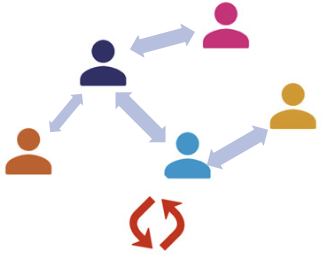
\includegraphics[width=3.38cm]{figures_zh/ch17/abm_people}};
  \node[inner sep=0pt] at (1.92,1.95)
    {
\includegraphics[width=3.28cm]{figures_zh/ch17/abm_environments}};
  \node[font=\fontsize{8}{10}\selectfont] at (.56,1.36) {物理};
  \node[font=\fontsize{8}{10}\selectfont] at (1.48,1.36) {社会};
  \node[font=\fontsize{8}{10}\selectfont] at (2.35,1.36) {网络};
  \node[font=\fontsize{8}{10}\selectfont] at (3.23,1.36) {混合};
  \node[req] (abm-social) at (5.38,5.55) {社会能力};
  \node[req] (abm-autonomy) at (5.38,4.22) {自主性};
  \node[req] (abm-reactivity) at (5.38,2.89) {反应性};
  \node[req] (abm-proactive) at (5.38,1.56) {主动性};
  \node[ability] (abm-perception) at (8.92,5.55) {感知};
  \node[ability] (abm-reason) at (8.92,4.22) {推理};
  \node[ability] (abm-decision) at (8.92,2.89) {决策};
  \node[ability] (abm-evolution) at (8.92,1.56) {自我演化};
  \foreach \from/\to in {perception/social,reason/social,
    reason/reactivity,decision/autonomy,decision/proactive,
    evolution/proactive}
    \draw[dashed,->] (abm-\from.west) -- (abm-\to.east);
  \draw[dashed,<->] (abm-reason.west) -- (abm-autonomy.east);
  \draw[dashed,<->] (abm-decision.west) -- (abm-reactivity.east);
  \draw[decorate,decoration={brace,amplitude=6pt}] (4.10,1.43) -- (4.10,5.53);
  \draw[decorate,decoration={brace,amplitude=6pt}] (10.38,5.58) -- (10.38,1.43);
  \draw[densely dotted,thick] (10.77,1.02) rectangle (15.52,5.98);
  \node[inner sep=0pt] at (11.60,3.60)
    {
\includegraphics[width=1.45cm]{figures_zh/ch17/abm_robot}};
  \node[font=\fontsize{7}{9}\selectfont] at (11.60,2.48) {大语言模型};
  \foreach \name/\y/\txt in {interface/5.12/接口,mechanism/3.58/内部机制,action/2.02/动作}
    \node[draw=blue!40!black,fill=orange!70!brown,text=white,ellipse,
      minimum width=2.50cm,minimum height=.72cm,font=\small] (abm-\name) at (14.03,\y) {\txt};
  \draw[->,orange!80!black,line width=1.5pt] (abm-interface.south) -- (abm-mechanism.north);
  \draw[->,orange!80!black,line width=1.5pt] (abm-mechanism.south) -- (abm-action.north);
  \node[font=\small\bfseries,align=center] at (3.48,.40) {基于智能体的建模\\与模拟的要求};
  \node[font=\small\bfseries,align=center] at (11.04,.40) {大语言模型\\智能体的能力};
\end{tikzpicture}

    \caption{基于智能体的建模与大语言模型智能体 \citep{gao2024large}}\label{fig:abm}
  \end{center}
\end{figure}

\begin{figure}
  \begin{center}
    \begin{tikzpicture}[x=1cm,y=1cm,>=Stealth,font=\small,
  cell/.style={draw,fill=white,minimum height=.48cm,align=center},
  fat/.style={->,line width=1.2pt},
  hollow/.style={->,draw=black!70,line width=3pt}]
  \path[use as bounding box] (0,0) rectangle (15.55,8.65);
  \node[cell,fill=blue!10,minimum width=1.30cm,minimum height=1.03cm] (st-data) at (.75,7.58) {真实\\数据};
  \node[cell,minimum width=2.80cm,minimum height=.65cm,font=\bfseries] (st-envtitle) at (3.35,7.84) {环境};
  \draw[hollow] (st-data.east) -- (st-envtitle.west);
  \draw[thick] (1.78,3.72) rectangle (4.92,7.32);
  \foreach \name/\y/\txt in {users/6.91/用户,messages/6.21/消息,network/5.51/网络}
    \node[cell,minimum width=2.72cm] (st-\name) at (3.35,\y) {\txt};
  \node[inner sep=0pt] at (3.35,4.47)
    {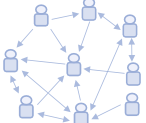
\includegraphics[height=1.45cm]{figures_zh/ch17/struct_network}};
  \node[text=red!75!black,font=\bfseries] at (5.22,8.44) {感知};
  \draw[hollow] (5.18,7.22) -- (5.72,7.22);
  \draw[thick] (6.05,3.95) rectangle (12.53,8.18);
  \node[cell,minimum width=2.15cm,minimum height=.63cm] (st-prompt) at (8.20,7.62) {提示设计};
  \node[cell,minimum width=2.15cm,minimum height=.63cm] (st-tuning) at (10.55,7.62) {调优};
  \node[text=red!75!black,font=\bfseries,align=center] at (13.65,7.66) {异质性\\与个性化};
  \node[draw=blue!50!black,fill=blue!10,minimum width=5.55cm,minimum height=.85cm,font=\bfseries]
    at (9.26,6.48) {大语言模型驱动的智能体};
  \draw[rounded corners=9pt,thick] (6.36,4.18) rectangle (12.08,5.72);
  \node[fill=blue!12,rounded corners=3pt,minimum width=3.35cm,minimum height=.57cm] at (9.28,5.77) {内部状态};
  \node[inner sep=0pt] at (7.13,5.77) {
\includegraphics[height=.83cm]{figures_zh/ch17/struct_person}};
  \foreach \x/\txt in {7.42/情绪,9.30/态度,11.13/其他}
    \node[cell,minimum width=1.53cm,minimum height=.57cm] at (\x,4.74) {\txt};
  \draw[hollow] (9.25,3.84) -- (9.25,3.22);
  \node[text=red!75!black,font=\fontsize{8.5}{10}\selectfont\bfseries] at (10.99,3.51) {推理与决策};
  \node[cell,fill=blue!9,minimum width=5.55cm,minimum height=.68cm,font=\bfseries] (st-gen) at (9.25,2.83) {生成模块};
  \node[cell,minimum width=1.90cm,minimum height=.63cm,text=blue!45,font=\bfseries] (st-cond) at (3.35,2.81) {条件};
  \draw[hollow] (st-cond.north) -- (3.35,3.64);
  \draw[hollow] (4.76,2.83) -- (6.24,2.83);
  \draw[thick] (1.90,.19) rectangle (4.87,2.25);
  \foreach \y/\txt in {1.80/社会事件,1.15/机制,.50/其他}
    \node[cell,minimum width=2.57cm] at (3.38,\y) {\txt};
  \draw[hollow] (9.25,2.35) -- (9.25,1.83);
  \draw[rounded corners=8pt,thick] (5.44,.27) rectangle (13.23,1.50);
  \node[fill=blue!12,rounded corners=3pt,minimum width=4.40cm,minimum height=.60cm] at (9.25,1.61) {交互行为};
  \node[inner sep=0pt] at (6.86,1.62) {
\includegraphics[height=.83cm]{figures_zh/ch17/struct_person}};
  \foreach \x/\txt/\wid in {6.24/点赞/1.00,7.97/转发/1.45,9.94/评论/1.66,11.93/生成/1.63}
    \node[cell,minimum width=\wid cm,minimum height=.57cm] at (\x,.84) {\txt};
  \draw[fat] (9.25,.27) -- (9.25,-.08) -- (.93,-.08) -- (.93,5.37) -- (1.78,5.37);
  \node[fill=white,align=center,font=\bfseries] at (.94,3.42) {环境\\更新};
  \draw[fat] (9.25,-.08) -- (13.88,-.08) -- (13.88,6.08) -- (12.53,6.08);
  \node[fill=white,text=blue!45,align=center,font=\bfseries] at (13.87,3.14) {记忆\\更新};
  \node[text=red!75!black,align=center,font=\bfseries] at (14.73,1.71) {适应性\\学习\\与演化};
\end{tikzpicture}

    \caption{用于多智能体建模的大语言模型智能体结构 \citep{gao2023s}}\label{fig:struct}
  \end{center}
\end{figure}

\subsection{从基于智能体的建模到生成式智能体社会}
对相互交互的人工智能体群体的研究，已有数十年历史。在基于智能体的建模（agent-based modeling，ABM）中，宏观层面的模式与规律由简单智能体的局部交互自下而上地产生 \citep{epstein1996growing, macal_tutorial_2010}。这一领域最有影响力的发现之一，是合作与规范能够在自利智能体群体中涌现 \citep{axelrod1986evolutionary}。文化演化（cultural evolution）理论将行为如何通过模仿、交流与教育在群体中传播加以形式化 \citep{boyd1988culture}。\citet{steels1995self} 的\emph{命名博弈（naming game）}表明，即使没有集中协调，共享词表也可以通过两两交互形成，而共享词表本质上也是一种惯例。

在经典的基于智能体的模拟中，智能体遵循手工编写的规则，交换抽象信息，而不会像本章中的智能体那样使用自然语言。另一个关键区别在于，经典智能体并不具备任何足以与大语言模型智能体相比的世界背景知识。
大语言模型使模拟进入了一个全然不同的层次：具有丰富多样角色设定的智能体会闲聊、劝说、误解和协商，其方式是人类一看就能理解的。模拟基础设施的进步，使得在群体规模上运行这类智能体成为可能 \citep{gao2024large, yang2024oasis}。由此形成的新一代\emph{生成式智能体社会（generative agent society）}，为既有的基于智能体的建模研究议程注入了新动力，同时也带来了新的方法学问题与考量。

在第~\ref{fivedimensions}~节中，我们介绍了用于描述多大语言模型系统研究控制程度的五轴谱系 \citep{tran2025multi}。基于角色的模拟与开放式模拟之间，是程度上的差异，而非本质上的区别。开放式模拟处在这一谱系的一端，与角色明确、协议化的交互相对。开放式模拟仍然包含为结果埋下种子的设计选择，但其决定性较弱，有意为新模式的涌现留下空间。这也改变了研究重心：研究不再围绕任务或明确目标评估表现，而是以开放视角展开，交互模式本身就是研究目标。开放式模拟更接近民族志研究，通过观察与探索来考察智能体如何行动和交互，因此需要不同的方法。下面我们将讨论这一点。

\subsection{方法学说明}\label{sec:meth-emergent}
第~\ref{chap:behavior}~章和第~\ref{chap:role}~章讨论的方法学问题，同样适用于开放式环境：提示敏感性、不同运行之间的变异、级联幻觉、弱点的相互强化，以及从人类语境借用术语的效度，都给开放式模拟带来挑战。我们将看到，这种环境会放大某些问题，同时缓解另一些问题。例如，在没有协议约束每一次智能体交互时，单个智能体层面的细微变化，就可能使整个模拟走上不同的轨道。这既使开放式模拟富有趣味，也使其十分脆弱。开放式环境还引入了一个新问题：涌现与检索之间的界线可能很模糊。当开放式模拟中的大语言模型智能体收敛到某个规范时，我们无法确定，这个规范究竟是从它们的交互中\emph{全新产生}的，还是仅仅从预训练获得的世界知识中检索出来的。

\citet{mou2024individual}、\citet{savarimuthu2024harnessing} 和 \citet{xi2023rise} 对这一新兴领域作了全面综述。我们将在第~\ref{sec:emergentinfra}~节讨论基础设施与模拟平台，随后在第~\ref{sec:maswork}~节讨论惯例与规范的涌现，再在第~\ref{sec:openworld}~节讨论开放世界环境的重要性。最后，我们将在第~\ref{sec:emergentrisk}~节反思开放式环境的风险。
接下来的第~\ref{chap:generative_agents}~章将提供一个实践案例，让你亲自动手操作开放式模拟。

\section{模拟基础设施}\label{sec:emergentinfra}
开放式模拟需要相应的基础设施。一方面，这些设施要提供一个平台，让智能体能够在较长时间内持续交互与行动，同时记录研究数据。另一方面，它们应当为现象自下而上的发生和未知结构的涌现留出足够空间，而不应构成限制。本节聚焦于规模问题，从居住在虚拟小镇中的单个模拟社区，逐步介绍到拥有一百万个智能体的社会。

\subsection{小世界}\label{sec:gen-agent}
\citet{park2023generative} 提出了名为 Generative Agents 的系统。在这个环境中，用户可以与一个模拟小镇交互，小镇中生活着 25 个基于大语言模型的智能体。该系统基于此前提出的社会拟像（social simulacra）技术 \citep{park2022social}，为每个智能体赋予独特的角色设定与初始记忆。系统记录每个智能体在模拟中的全部经历与对话，并利用这些记录综合形成更高层次的反思，规划后续行为（见图~\ref{fig:simulacra1}）。

在 Generative Agents 中，智能体的行为有些像电子游戏 The Sims 中的人物 \citep{nutt2003sims}：它们会主动交谈、建立关系、传播信息，并协调临时性的群体活动（见图~\ref{fig:simulacra2}）。需要注意的是，交互受到用户输入的影响，因此具有半自主性；模拟在很大程度上没有预设脚本，但并非完全如此。情人节派对的例子展示了模拟如何运作：用户通过提示发起派对计划，随后多个智能体相互传递邀请，并协调各自的计划，在合适的时间到场，有的也会迟到，就像现实生活中一样。智能体形成了可信的社会日常活动，例如日程安排与闲聊，甚至表现出类似人类的性格特点：一些智能体表现出欺骗或固执，另一些则表现出合作。这些结果表明，只要给予合适的初始提示，社会模式就可能从动态、半自主的大语言模型交互中涌现。

\begin{figure}
  \begin{center}
    \begin{tikzpicture}[x=1cm,y=1cm,>=Stealth,font=\small,
  process/.style={draw,rounded corners=4pt,minimum width=1.85cm,minimum height=.72cm},
  store/.style={draw,minimum width=2.60cm,minimum height=1.06cm,font=\bfseries}]
  \path[use as bounding box] (0,0) rectangle (15.50,5.10);
  \draw[dashed,gray,thick] (2.35,1.25) rectangle (13.10,3.78);
  \node[fill=white,font=\bfseries] at (7.76,3.58) {生成式智能体记忆};
  \node[process] (sm-perceive) at (1.02,2.55) {感知};
  \node[store] (sm-memory) at (4.15,2.55) {记忆流};
  \draw[gray] (2.89,2.06) rectangle (5.41,3.04);
  \node[process] (sm-retrieve) at (7.76,2.55) {检索};
  \node[store] (sm-retrieved) at (11.36,2.55) {检索得到的记忆};
  \draw[gray] (10.10,2.06) rectangle (12.62,3.04);
  \node[process] (sm-act) at (14.49,2.55) {行动};
  \node[process] (sm-plan) at (7.76,4.62) {规划};
  \node[process] (sm-reflect) at (7.76,.48) {反思};
  \draw[->] (sm-perceive) -- (sm-memory);
  \draw[->] (sm-memory) -- (sm-retrieve);
  \draw[->] (sm-retrieve) -- (sm-retrieved);
  \draw[->] (sm-retrieved) -- (sm-act);
  \draw[->] (sm-retrieved.north) to[out=90,in=0] (sm-plan.east);
  \draw[->] (sm-plan.west) to[out=180,in=90] (sm-memory.north);
  \draw[->] (sm-retrieved.south) to[out=-90,in=0] (sm-reflect.east);
  \draw[->] (sm-reflect.west) to[out=180,in=-90] (sm-memory.south);
\end{tikzpicture}

    \caption{记忆—反思—规划循环是 Generative Agents 系统得以运作的关键设计：如果不能从持续增长的经历记录中检索，并定期反思，智能体就会在模拟时间的数小时内失去连贯性 \citep{park2023generative}}\label{fig:simulacra1}
  \end{center}
\end{figure}

\begin{figure}
  \begin{center}
    \begin{tikzpicture}[x=0.01372807cm,y=-0.01372807cm]
\path[use as bounding box] (0,0) rectangle (1140,612);
\node[anchor=north west,inner sep=0pt] at (0,0) {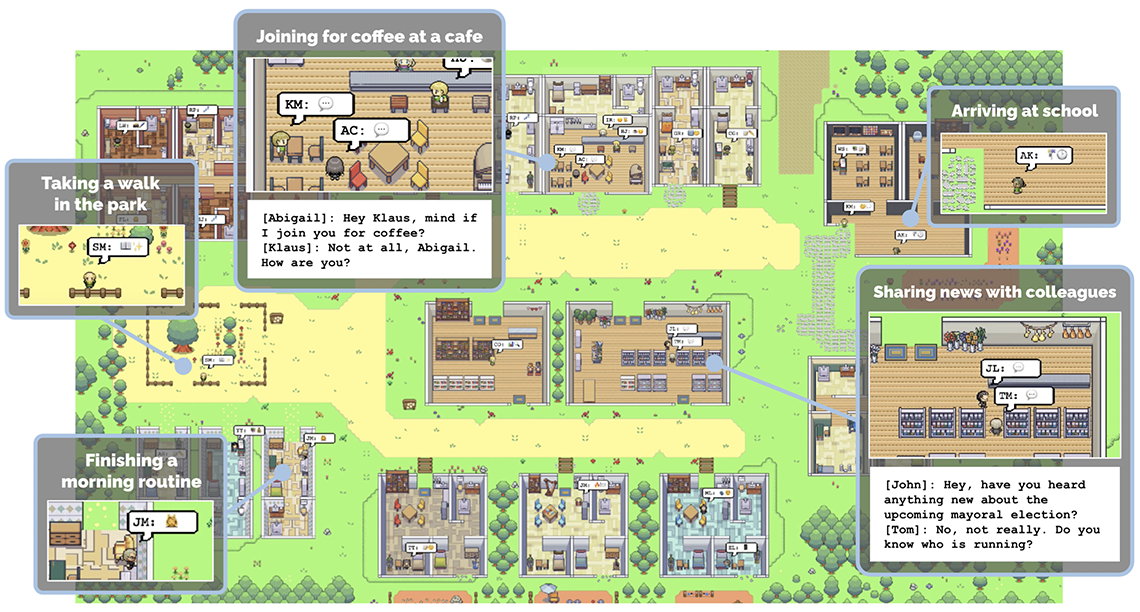
\includegraphics[width=15.65cm]{figures/simulacra2}};
\definecolor{chSeventeensimulacra20}{RGB}{145,147,145}
\fill[chSeventeensimulacra20] (242,16) rectangle (498,52);
\node[inner sep=0pt,align=center,text=white,text width=3.5144cm,font=\fontsize{8.3}{9.296000000000001}\selectfont\bfseries] at (370.0,34.0) {在咖啡馆一起喝咖啡};
\definecolor{chSeventeensimulacra21}{RGB}{145,147,145}
\fill[chSeventeensimulacra21] (15,170) rectangle (190,215);
\node[inner sep=0pt,align=center,text=white,text width=2.4024cm,font=\fontsize{8.3}{9.296000000000001}\selectfont\bfseries] at (102.5,192.5) {在公园散步};
\definecolor{chSeventeensimulacra22}{RGB}{145,147,145}
\fill[chSeventeensimulacra22] (41,445) rectangle (218,492);
\node[inner sep=0pt,align=center,text=white,text width=2.4299cm,font=\fontsize{8.0}{8.96}\selectfont\bfseries] at (129.5,468.5) {完成早晨的日常活动};
\definecolor{chSeventeensimulacra23}{RGB}{145,147,145}
\fill[chSeventeensimulacra23] (941,94) rectangle (1109,131);
\node[inner sep=0pt,align=center,text=white,text width=2.3063cm,font=\fontsize{8.3}{9.296000000000001}\selectfont\bfseries] at (1025.0,112.5) {到达学校};
\definecolor{chSeventeensimulacra24}{RGB}{145,147,145}
\fill[chSeventeensimulacra24] (866,275) rectangle (1124,310);
\node[inner sep=0pt,align=center,text=white,text width=3.5418cm,font=\fontsize{8.3}{9.296000000000001}\selectfont\bfseries] at (995.0,292.5) {与同事分享消息};
\definecolor{chSeventeensimulacra25}{RGB}{255,255,255}
\fill[chSeventeensimulacra25] (250,199) rectangle (491,281);
\node[inner sep=0pt,align=center,text=black,text width=3.3085cm,font=\fontsize{6.85}{6.9185}\selectfont] at (370.5,240.0) {[Abigail]：嘿，Klaus，我能\\和你一起喝杯咖啡吗？\\{}[Klaus]：当然可以，Abigail。\\你好吗？};
\definecolor{chSeventeensimulacra26}{RGB}{255,255,255}
\fill[chSeventeensimulacra26] (884,473) rectangle (1122,560);
\node[inner sep=0pt,align=center,text=black,text width=3.2673cm,font=\fontsize{7.0}{7.840000000000001}\selectfont] at (1003.0,516.5) {[John]：嘿，听说即将举行的\\市长选举有什么消息吗？\\{}[Tom]：不太清楚。你知道\\谁要参选吗？};
\end{tikzpicture}

    \caption{Generative Agents 模拟示例：包含 25 个智能体，并通过交互设计让用户能够启动其行为 \citep{park2023generative}}\label{fig:simulacra2}
  \end{center}
\end{figure}

\subsection{从数千个到一百万个智能体的社会}
将 Generative Agents 架构从 25 个智能体进一步扩展，会遇到推理成本问题，也会遇到如何构建足够丰富、能够容纳数千个智能体活动的环境的问题。\footnote{正如你将在下一章的动手实践中体验到的，即使运行一个只有三个活跃智能体的 Generative Agents 架构变体，计算上也已经颇具挑战。}大型社会模拟需要在可用算力、模拟总运行时间、智能体数量与单个智能体行为的准确性之间权衡。已有若干平台尝试应对这些问题。

AgentSociety 是一个包含超过 10,000 个智能体的大规模模拟系统 \citep{piao2025agentsociety}。它将大语言模型驱动的智能体与逼真的城市环境相结合，重点关注出行、就业与消费。它不仅像 Generative Agents 那样研究日常社会动态，还为计算社会实验提供试验平台。为了达到所需规模，模拟在分布式推理后端上运行，并对智能体行为实施更严格的控制。

OASIS 是一个面向 Twitter/X 和 Reddit、可扩展的社交媒体模拟器 \citep{yang2024oasis}，支持对多达一百万个大语言模型智能体进行建模。它构建于 CAMEL \citep{li2023camel} 之上，以基于角色的智能体为起点。在 OASIS 中，并非每个智能体动作都需要调用大语言模型，也并非所有智能体始终处于活跃状态。在这样的大规模下，OASIS 展现出多种社会群体现象，包括信息与错误信息的传播、群体极化和从众效应。OASIS 由环境服务器、推荐系统、智能体模块、时间引擎和可扩展推理器构成（见图~\ref{fig:oasis}）。

\begin{figure}
  \begin{center}
    \begin{tikzpicture}[x=1cm,y=1cm,>=Stealth,font=\fontsize{8}{9.2}\selectfont,
  workflow/.style={->,blue!75!black,line width=1.1pt},
  timeflow/.style={->,green!40!black,line width=1.1pt},
  recflow/.style={->,blue!55!black,line width=.7pt},
  card/.style={rounded corners=5pt,draw=none,fill=orange!13},
  queue/.style={draw=blue!65,dashed,rounded corners=3pt},
  module/.style={rounded corners=5pt,line width=.85pt}]
  \path[use as bounding box] (0,0) rectangle (15.55,21.15);
  \definecolor{ch17OaPeach}{RGB}{252,229,212}

  \draw[workflow] (.15,20.85) -- (1.15,20.85);
  \node[anchor=west] at (1.26,20.85) {工作流};
  \draw[timeflow] (3.05,20.85) -- (4.05,20.85);
  \node[anchor=west] at (4.16,20.85) {时间流};
  \draw[orange!80!black] (5.87,20.85) -- (6.70,20.85);
  \node[anchor=west] at (6.82,20.85) {关系};
  \node[inner sep=0pt] at (8.41,20.85) {
\includegraphics[width=.33cm]{figures_zh/ch17/oa_post_icon}};
  \node[anchor=west] at (8.74,20.85) {帖子};
  \node[inner sep=0pt] at (10.51,20.85) {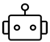
\includegraphics[width=.48cm]{figures_zh/ch17/oa_agent_icon}};
  \node[anchor=west] at (10.91,20.85) {智能体或用户};

  \node[inner sep=0pt] at (.80,19.62) {
\includegraphics[width=1.00cm]{figures_zh/ch17/oa_real_users}};
  \node[align=center,font=\fontsize{8}{9.2}\selectfont\bfseries] at (.80,18.75) {现实世界\\用户};
  \node[inner sep=0pt] at (3.11,19.72) {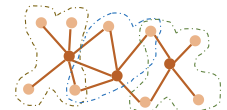
\includegraphics[width=2.30cm]{figures_zh/ch17/oa_generation}};
  \node at (3.11,19.04) {\#商业　\#体育　\#教育};
  \fill[orange!85!black] (2.02,18.72) circle (.045);
  \node[anchor=west,font=\fontsize{7}{8}\selectfont] at (2.11,18.72) {核心用户};
  \fill[orange!40] (3.25,18.72) circle (.045);
  \node[anchor=west,font=\fontsize{7}{8}\selectfont] at (3.34,18.72) {普通用户};
  \node[font=\fontsize{8}{9.2}\selectfont\bfseries] at (3.11,18.32) {大规模用户生成};
  \draw[workflow] (3.11,18.10) -- node[right] {注册} (3.11,16.94);

  \node[font=\fontsize{8}{9.2}\selectfont\bfseries,text=orange!80!black] (oa-env-overview) at (5.80,18.24) {环境服务器};
  \node[font=\fontsize{8}{9.2}\selectfont\bfseries,text=blue!60!black] (oa-rec-overview) at (8.51,18.24) {推荐系统};
  \node[font=\fontsize{8}{9.2}\selectfont\bfseries,text=yellow!40!black] (oa-agent-overview) at (10.96,18.24) {智能体};
  \node[font=\fontsize{8}{9.2}\selectfont\bfseries,text=green!40!black] (oa-time-overview) at (14.19,18.24) {时间引擎};
  \draw[workflow] (5.80,19.20) -- node[left] {注册} (oa-env-overview.north);
  \draw[workflow] (oa-env-overview.east) -- node[above,align=center,font=\fontsize{7}{8}\selectfont]
    {用户信息、帖子\\信息与关系} (oa-rec-overview.west);
  \draw[workflow] (oa-rec-overview.east) -- node[above,font=\fontsize{7}{8}\selectfont]
    {筛选后的帖子} (oa-agent-overview.west);
  \draw[workflow] (oa-agent-overview.north) -- (10.96,19.38) --
    node[above] {动作} (6.55,19.38) -- (oa-env-overview.north east);
  \draw[timeflow] (oa-time-overview.west) -- node[above] {激活} (oa-agent-overview.east);
  \draw[timeflow] (12.46,18.52) -- (12.46,20.25);
  \draw[green!40!black,thick] (12.27,19.25) -- (12.46,19.25);
  \draw[green!40!black,thick] (12.27,19.77) -- (12.46,19.77);
  \node[anchor=west,font=\fontsize{7}{8}\selectfont,text=green!40!black] at (12.53,19.25) {下午1时};
  \node[anchor=west,font=\fontsize{7}{8}\selectfont,text=green!40!black] at (12.53,19.77) {下午2时};
  \node[inner sep=0pt] at (14.34,19.75) {
\includegraphics[width=1.45cm]{figures_zh/ch17/oa_frequency}};
  \node[align=center,font=\fontsize{7.3}{8.3}\selectfont] at (14.32,19.00) {不同时段的\\交互频率};
  \draw[timeflow] (14.19,18.78) -- node[right,font=\fontsize{7}{8}\selectfont] {初始化} (oa-time-overview.north);

  \draw[module,orange!80!black] (.10,9.10) rectangle (6.68,16.94);
  \node[font=\small\bfseries,text=orange!80!black,fill=white] at (1.65,16.94) {环境服务器};
  \fill[card] (.28,13.65) rectangle (6.47,16.55);
  \node[anchor=west,text=orange!80!black,font=\bfseries] at (.49,16.22) {用户};
  \node[inner sep=0pt] at (1.10,14.93) {
\includegraphics[height=1.79cm]{figures_zh/ch17/oa_user_pair}};
  \node[align=left,anchor=west,text width=4.38cm] at (1.84,15.40) {姓名｜简介｜关注者列表……};
  \node[align=left,anchor=west,text width=4.38cm] at (1.84,14.51) {姓名｜简介｜关注者列表……};
  \node[anchor=west] at (.57,13.93) {$\cdots$};

  \fill[card] (.28,10.99) rectangle (6.47,13.36);
  \node[anchor=west,text=orange!80!black,font=\bfseries] at (.49,13.08) {帖子};
  \node[inner sep=0pt] at (.85,12.42) {
\includegraphics[width=.63cm]{figures_zh/ch17/oa_post1}};
  \node[anchor=west] at (1.31,12.42) {真不错……};
  \node[inner sep=0pt] at (4.87,12.42) {
\includegraphics[width=2.25cm]{figures_zh/ch17/oa_counts1}};
  \node[inner sep=0pt] at (.85,11.66) {
\includegraphics[width=.63cm]{figures_zh/ch17/oa_post2}};
  \node[anchor=west] at (1.31,11.66) {这是一个……};
  \node[inner sep=0pt] at (4.87,11.66) {
\includegraphics[width=2.25cm]{figures_zh/ch17/oa_counts2}};
  \node[anchor=west] at (.57,11.21) {$\cdots$};

  \fill[card] (.28,9.34) rectangle (6.47,10.74);
  \node[anchor=west,text=orange!80!black,font=\bfseries] at (.49,10.47) {动态智能体网络};
  \node[inner sep=0pt] at (1.26,9.86) {
\includegraphics[width=1.05cm]{figures_zh/ch17/oa_network_before_clean}};
  \node[inner sep=0pt] at (4.93,9.86) {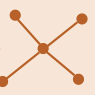
\includegraphics[width=1.05cm]{figures_zh/ch17/oa_network_after}};
  \draw[->,orange!80!black] (2.08,9.87) -- node[above] {更新} (4.10,9.87);
  \node[anchor=west] at (.57,9.16) {$\cdots$};

  \draw[module,blue!65] (8.19,9.10) rectangle (15.48,16.94);
  \node[font=\small\bfseries,text=blue!60!black,fill=white] at (10.08,16.94) {推荐系统};
  \draw[workflow] (6.68,15.13) -- node[above,font=\fontsize{7}{8}\selectfont,text=orange!80!black] {用户信息} (8.19,15.13);
  \draw[workflow] (6.68,12.34) -- node[above,font=\fontsize{7}{8}\selectfont,text=orange!80!black] {帖子信息} (8.19,12.34);
  \draw[workflow] (6.68,10.10) -- node[above,font=\fontsize{7}{8}\selectfont,text=orange!80!black] {关系} (8.19,10.10);
  \node[inner sep=0pt] at (9.88,15.02) {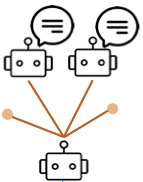
\includegraphics[height=2.75cm]{figures_zh/ch17/oa_rec_agents_clean}};
  \node[inner sep=0pt] at (13.65,15.46) {
\includegraphics[width=2.25cm]{figures_zh/ch17/oa_rec_pool}};
  \draw[recflow] (13.65,14.39) -- (13.65,14.11);
  \node[draw=blue!60!black,rounded corners=2pt,text=blue!60!black,minimum width=2.50cm,minimum height=.37cm]
    (oa-interest) at (13.65,13.87) {兴趣匹配};
  \draw[recflow] (oa-interest.south) -- (13.65,13.40);
  \draw[recflow] (9.88,13.62) -- (9.88,13.40);
  \draw[queue] (8.73,12.55) rectangle (11.03,13.38);
  \node[inner sep=0pt] at (9.88,12.96) {
\includegraphics[width=1.77cm]{figures_zh/ch17/oa_rec_in}};
  \node[text=blue!60!black,font=\bfseries] at (9.88,12.24) {网络内};
  \draw[queue] (12.50,12.55) rectangle (14.80,13.38);
  \node[inner sep=0pt] at (13.65,12.96) {
\includegraphics[width=1.77cm]{figures_zh/ch17/oa_rec_out}};
  \node[text=blue!60!black,font=\bfseries] at (13.65,12.24) {网络外};
  \draw[queue] (10.61,11.44) rectangle (12.91,12.26);
  \node[inner sep=0pt] at (11.76,11.85) {
\includegraphics[width=1.77cm]{figures_zh/ch17/oa_rec_hot}};
  \node[text=blue!60!black,font=\bfseries] at (11.76,11.20) {热度得分};
  \node[inner sep=0pt] at (11.76,10.10) {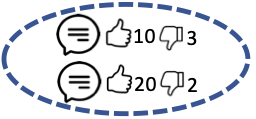
\includegraphics[width=3.50cm]{figures_zh/ch17/oa_rec_scores}};
  \draw[recflow] (11.76,10.91) -- (11.76,11.04);

  \draw[workflow] (11.76,9.10) -- (11.76,8.69) -- (3.73,8.69) -- (3.73,8.34);
  \node[fill=white] at (7.74,8.69) {筛选后的帖子};

  \draw[module,yellow!60!black] (.10,.50) rectangle (7.42,8.34);
  \node[font=\small\bfseries,text=yellow!40!black,fill=white] at (1.67,8.34) {智能体模块};
  \node[text=blue!60!black,font=\bfseries] at (2.77,7.76) {筛选帖子};
  \node[text=orange!80!black,font=\bfseries] at (5.00,7.76) {智能体信息};
  \draw[->,yellow!60!black] (3.73,7.49) -- (3.73,7.14);
  \node[inner sep=0pt] at (3.73,6.67) {
\includegraphics[width=1.02cm]{figures_zh/ch17/oa_memory}};
  \node[font=\bfseries,text=yellow!40!black] at (3.73,5.99) {记忆};
  \draw[->,yellow!60!black] (3.73,5.74) -- (3.73,5.40);
  \node[inner sep=0pt] at (2.70,4.89) {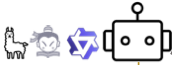
\includegraphics[width=3.39cm]{figures_zh/ch17/oa_models_agent}};
  \node[inner sep=0pt] at (1.29,4.10) {
\includegraphics[width=.53cm]{figures_zh/ch17/oa_openai}};
  \node[font=\bfseries,text=yellow!40!black] at (2.18,4.10) {LLM};
  \draw[->,yellow!60!black] (3.73,4.29) -- (3.73,3.90);
  \node[align=center,font=\bfseries] at (1.30,3.38) {这真让我\\感兴趣！};
  \node[font=\bfseries,text=yellow!40!black] at (1.30,2.71) {理由};
  \draw[dashed,yellow!60!black,rounded corners=3pt] (3.00,2.50) rectangle (6.67,3.90);
  \node[inner sep=0pt] at (4.84,3.48) {
\includegraphics[width=3.08cm]{figures_zh/ch17/oa_actions}};
  \node[font=\fontsize{7.5}{8.5}\selectfont,text=yellow!40!black] at (3.68,2.86) {发帖};
  \node[font=\fontsize{7.5}{8.5}\selectfont,text=yellow!40!black] at (4.46,2.86) {点赞};
  \node[font=\fontsize{7.5}{8.5}\selectfont,text=yellow!40!black] at (5.45,2.86) {评论};
  \node[font=\bfseries,text=yellow!40!black] at (4.84,2.15) {动作};
  \draw[workflow] (4.84,1.85) -- (4.84,1.34);
  \node[font=\bfseries,text=orange!80!black] at (4.84,.94) {环境服务器};
  \node[inner sep=0pt] at (1.87,1.05) {
\includegraphics[width=2.69cm]{figures_zh/ch17/oa_logo}};

  \draw[module,green!35!black] (8.19,4.47) rectangle (15.48,8.34);
  \node[font=\small\bfseries,text=green!35!black,fill=white] at (9.74,8.34) {时间引擎};
  \draw[timeflow] (9.48,5.15) -- (9.48,7.91);
  \draw[green!40!black] (9.32,7.31) -- (9.48,7.31);
  \fill[green!40!black] (9.48,5.91) circle (.08);
  \node[anchor=east,text=green!40!black] at (9.21,7.31) {下午2时};
  \node[anchor=east,text=green!40!black] at (9.21,5.91) {下午1时};
  \node[inner sep=0pt] at (8.92,5.18) {
\includegraphics[width=.50cm]{figures_zh/ch17/oa_clock}};
  \node[inner sep=0pt] at (12.67,6.71) {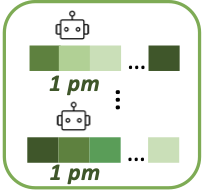
\includegraphics[width=3.15cm]{figures_zh/ch17/oa_time_queues}};
  \fill[white] (11.73,6.68) rectangle (12.96,7.10);
  \node[text=green!35!black] at (12.34,6.89) {下午1时};
  \fill[white] (11.73,5.28) rectangle (12.96,5.72);
  \node[text=green!35!black] at (12.34,5.50) {下午1时};
  \node[inner sep=0pt] at (12.67,4.73) {
\includegraphics[width=3.50cm]{figures_zh/ch17/oa_active_bar_clean}};
  \node[font=\bfseries] at (12.71,4.73) {活跃程度};
  \draw[timeflow] (8.19,6.05) -- node[above,sloped,fill=white] {激活} (4.35,4.98);

  \draw[module,gray] (8.19,.50) rectangle (15.48,3.96);
  \node[font=\small\bfseries,text=gray,fill=white] at (10.41,3.96) {可扩展推理器};
  \node[inner sep=0pt] at (11.83,2.23) {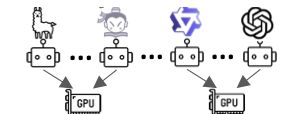
\includegraphics[width=6.52cm]{figures_zh/ch17/oa_inferencer_clean}};
  \draw[->,gray,line width=.8pt] (12.41,.87) -- (13.87,.87);
  \node[text=gray,anchor=west] at (14.04,.87) {线程};
  \draw[->,gray,line width=1.15pt] (4.35,4.71) --
    node[above,sloped,fill=white] {推理} (7.82,4.22) -- (8.19,2.55);
\end{tikzpicture}

    \caption{OASIS 的组成部分 \citep{yang2024oasis}}\label{fig:oasis}
  \end{center}
\end{figure}

Project Sid \citep{al2024projectsid} 将多达 1000 个智能体放入 Minecraft 世界，并报告了一项引人注目的涌现结果：研究者观察到，智能体发展出专门的经济角色，如农民、矿工与守卫，遵守共同采纳的规则，如税收，并在聚居地之间传播文化模因，甚至宗教模因。不过，尽管交互没有预设脚本，前文提出的涌现与检索之辨在这里依然适用：可以预期，驱动这些智能体的大语言模型，其训练数据已经大量描述了所观察到的角色与行为。

\subsection{作为科学工具的模拟}
这些平台不仅是可扩展大语言模型技术令人印象深刻的展示；只要谨慎使用，它们也可用于复杂的计算社会实验。研究者已经利用模拟的生成式智能体社会，研究社会科学中的长期问题（第~\ref{sec:interacting}~节）。例如，AgentSociety 被用于多种案例研究，包括煽动性消息的传播、极化、全民基本收入政策的效果，以及飓风等外部冲击对社会的影响 \citep{piao2025agentsociety, piao2025polarization}。在人类群体中开展这类实验，可能不符合伦理、不切实际，甚至根本不可能。作者指出，在模拟中，这些实验可以重复开展，也可以在每一步修改实验。

\citet{li2024large} 进一步以错误信息为例展示了这种方法。他们的智能体在性别、年龄和大五人格特征上具有多样化的设定。\footnote{也称 OCEAN：开放性（Openness）、尽责性（Conscientiousness）、外向性（Extraversion）、宜人性（Agreeableness）和神经质（Neuroticism）。}其中一项发现是，鼓励评论并不能显著减少错误信息的传播；相比之下，公开为信息标注准确性得分，以及屏蔽特定的意见领袖，被证明是有效策略，尤其是在无标度网络（scale-free network）中 \citep{barabasi2009scale}。这类研究有一种典型模式：把候选干预措施实现为模拟平台的一项改动，并通过多次运行测量其宏观效果。这些效果能否迁移到人类群体，正是第~\ref{sec:meth-emergent}~节所讨论的效度问题。对于此类模拟，最合适的理解是把它们视为生成假设和开展预试验的工具，而不是实地实验的替代品。

\paragraph{一个边界案例：AgentVerse}
严格来说，AgentVerse \citep{chen2023agentverse} 属于第~\ref{chap:role}~章研究的那类基于角色的系统。AgentVerse 将问题求解分为四个阶段：招募专家、协作决策、执行动作和评估，并不断迭代，直到结果令人满意（图~\ref{fig:agentverse}）。我们在这里提到它，是因为系统中发生了\emph{超出}设计的行为：智能体表现出主动提供帮助的涌现行为，即主动为同伴提供协助；也表现出从众，即在他人的批评下调整偏离群体的行为。研究者还观察到了破坏性行为，偶尔造成不期望出现的有害结果。在预设角色的模拟中出现宏观行为，说明基于角色的交互与涌现之间存在一个连续谱：即使系统受到严密协议的约束，也经常表现出无人刻意设计的行为。第~\ref{sec:emergentrisk}~节将再讨论这一现象涉及的风险。

\begin{figure}
  \begin{center}
    \begin{tikzpicture}[x=0.00908827cm,y=-0.00908827cm]
\path[use as bounding box] (0,0) rectangle (1722,946);
\node[anchor=north west,inner sep=0pt] at (0,0) {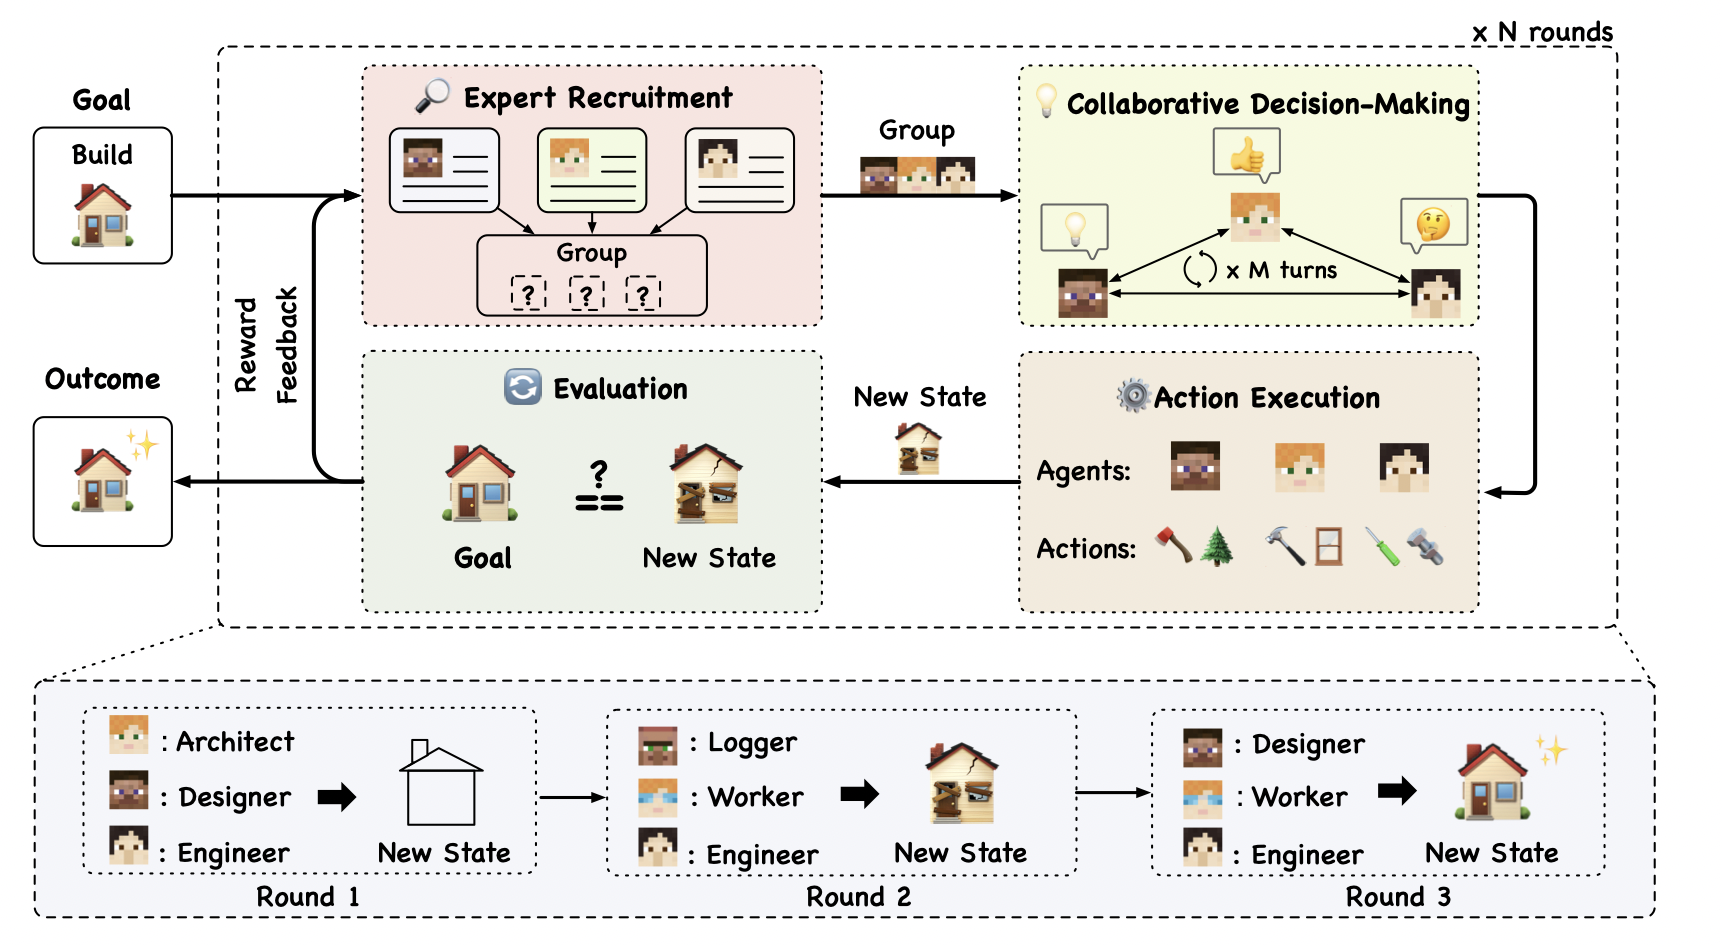
\includegraphics[width=15.65cm]{figures/agentverse}};
\definecolor{chSeventeenagentverse0}{RGB}{255,255,255}
\fill[chSeventeenagentverse0] (1467,14) rectangle (1610,45);
\node[inner sep=0pt,align=center,text=black,text width=1.2996cm,font=\fontsize{8.1}{9.072000000000001}\selectfont\bfseries] at (1538.5,29.5) {× N 轮};
\definecolor{chSeventeenagentverse1}{RGB}{255,255,255}
\fill[chSeventeenagentverse1] (65,79) rectangle (138,115);
\node[inner sep=0pt,align=center,text=black,text width=0.6634cm,font=\fontsize{9.2}{10.304}\selectfont\bfseries] at (101.5,97.0) {目标};
\definecolor{chSeventeenagentverse2}{RGB}{255,255,255}
\fill[chSeventeenagentverse2] (67,141) rectangle (138,171);
\node[inner sep=0pt,align=center,text=black,text width=0.6453cm,font=\fontsize{8.7}{9.744}\selectfont\bfseries] at (102.5,156.0) {建造};
\definecolor{chSeventeenagentverse3}{RGB}{255,255,255}
\fill[chSeventeenagentverse3] (40,361) rectangle (167,396);
\node[inner sep=0pt,align=center,text=black,text width=1.1542cm,font=\fontsize{9.2}{10.304}\selectfont\bfseries] at (103.5,378.5) {结果};
\definecolor{chSeventeenagentverse4}{RGB}{250,230,226}
\fill[chSeventeenagentverse4] (457,79) rectangle (793,117);
\node[inner sep=0pt,align=center,text=black,text width=3.0537cm,font=\fontsize{9.2}{10.304}\selectfont\bfseries] at (625.0,98.0) {招募专家};
\definecolor{chSeventeenagentverse5}{RGB}{248,251,222}
\fill[chSeventeenagentverse5] (1065,78) rectangle (1470,122);
\node[inner sep=0pt,align=center,text=black,text width=3.6807cm,font=\fontsize{9.2}{10.304}\selectfont\bfseries] at (1267.5,100.0) {协作决策};
\definecolor{chSeventeenagentverse6}{RGB}{250,230,226}
\fill[chSeventeenagentverse6] (549,241) rectangle (650,267);
\node[inner sep=0pt,align=center,text=black,text width=0.9179cm,font=\fontsize{8.2}{9.184}\selectfont\bfseries] at (599.5,254.0) {团队};
\definecolor{chSeventeenagentverse7}{RGB}{255,255,255}
\fill[chSeventeenagentverse7] (875,112) rectangle (963,146);
\node[inner sep=0pt,align=center,text=black,text width=0.7998cm,font=\fontsize{8.7}{9.744}\selectfont\bfseries] at (919.0,129.0) {团队};
\definecolor{chSeventeenagentverse8}{RGB}{248,251,222}
\fill[chSeventeenagentverse8] (1222,252) rectangle (1347,283);
\node[inner sep=0pt,align=center,text=black,text width=1.1360cm,font=\fontsize{7.5}{8.4}\selectfont] at (1284.5,267.5) {× M 回合};
\definecolor{chSeventeenagentverse9}{RGB}{236,242,232}
\fill[chSeventeenagentverse9] (551,367) rectangle (701,411);
\node[inner sep=0pt,align=center,text=black,text width=1.3632cm,font=\fontsize{9.2}{10.304}\selectfont\bfseries] at (626.0,389.0) {评估};
\definecolor{chSeventeenagentverse10}{RGB}{246,237,222}
\fill[chSeventeenagentverse10] (1154,373) rectangle (1418,416);
\node[inner sep=0pt,align=center,text=black,text width=2.3993cm,font=\fontsize{9.2}{10.304}\selectfont\bfseries] at (1286.0,394.5) {执行动作};
\definecolor{chSeventeenagentverse11}{RGB}{255,255,255}
\fill[chSeventeenagentverse11] (849,379) rectangle (993,414);
\node[inner sep=0pt,align=center,text=black,text width=1.3087cm,font=\fontsize{8.7}{9.744}\selectfont\bfseries] at (921.0,396.5) {新状态};
\definecolor{chSeventeenagentverse12}{RGB}{246,237,222}
\fill[chSeventeenagentverse12] (1033,452) rectangle (1158,490);
\node[inner sep=0pt,align=center,text=black,text width=1.1360cm,font=\fontsize{8.0}{8.96}\selectfont] at (1095.5,471.0) {智能体：};
\definecolor{chSeventeenagentverse13}{RGB}{246,237,222}
\fill[chSeventeenagentverse13] (1031,530) rectangle (1140,569);
\node[inner sep=0pt,align=center,text=black,text width=0.9906cm,font=\fontsize{8.5}{9.520000000000001}\selectfont] at (1085.5,549.5) {动作：};
\definecolor{chSeventeenagentverse14}{RGB}{236,242,232}
\fill[chSeventeenagentverse14] (450,537) rectangle (520,574);
\node[inner sep=0pt,align=center,text=black,text width=0.6362cm,font=\fontsize{8.5}{9.520000000000001}\selectfont\bfseries] at (485.0,555.5) {目标};
\definecolor{chSeventeenagentverse15}{RGB}{236,242,232}
\fill[chSeventeenagentverse15] (643,538) rectangle (790,575);
\node[inner sep=0pt,align=center,text=black,text width=1.3360cm,font=\fontsize{8.5}{9.520000000000001}\selectfont\bfseries] at (716.5,556.5) {新状态};
\definecolor{chSeventeenagentverse16}{RGB}{255,255,255}
\fill[chSeventeenagentverse16] (222,278) rectangle (304,422);
\node[inner sep=0pt,align=center,text=black,text width=1.2669cm,font=\fontsize{8.0}{8.96}\selectfont,rotate=90] at (263.0,350.0) {奖励反馈};
\definecolor{chSeventeenagentverse17}{RGB}{244,245,249}
\fill[chSeventeenagentverse17] (168,725) rectangle (307,759);
\node[inner sep=0pt,align=center,text=black,text width=1.2633cm,font=\fontsize{8.0}{8.96}\selectfont] at (237.5,742.0) {：建筑师};
\definecolor{chSeventeenagentverse18}{RGB}{244,245,249}
\fill[chSeventeenagentverse18] (168,778) rectangle (307,812);
\node[inner sep=0pt,align=center,text=black,text width=1.2633cm,font=\fontsize{8.0}{8.96}\selectfont] at (237.5,795.0) {：设计师};
\definecolor{chSeventeenagentverse19}{RGB}{244,245,249}
\fill[chSeventeenagentverse19] (168,830) rectangle (307,863);
\node[inner sep=0pt,align=center,text=black,text width=1.2633cm,font=\fontsize{8.0}{8.96}\selectfont] at (237.5,846.5) {：工程师};
\definecolor{chSeventeenagentverse20}{RGB}{244,245,249}
\fill[chSeventeenagentverse20] (376,836) rectangle (514,872);
\node[inner sep=0pt,align=center,text=black,text width=1.2542cm,font=\fontsize{8.2}{9.184}\selectfont\bfseries] at (445.0,854.0) {新状态};
\definecolor{chSeventeenagentverse21}{RGB}{244,245,249}
\fill[chSeventeenagentverse21] (695,727) rectangle (831,761);
\node[inner sep=0pt,align=center,text=black,text width=1.2360cm,font=\fontsize{8.0}{8.96}\selectfont] at (763.0,744.0) {：伐木工};
\definecolor{chSeventeenagentverse22}{RGB}{244,245,249}
\fill[chSeventeenagentverse22] (695,779) rectangle (831,812);
\node[inner sep=0pt,align=center,text=black,text width=1.2360cm,font=\fontsize{8.0}{8.96}\selectfont] at (763.0,795.5) {：工人};
\definecolor{chSeventeenagentverse23}{RGB}{244,245,249}
\fill[chSeventeenagentverse23] (695,832) rectangle (831,866);
\node[inner sep=0pt,align=center,text=black,text width=1.2360cm,font=\fontsize{8.0}{8.96}\selectfont] at (763.0,849.0) {：工程师};
\definecolor{chSeventeenagentverse24}{RGB}{244,245,249}
\fill[chSeventeenagentverse24] (895,838) rectangle (1040,874);
\node[inner sep=0pt,align=center,text=black,text width=1.3178cm,font=\fontsize{8.2}{9.184}\selectfont\bfseries] at (967.5,856.0) {新状态};
\definecolor{chSeventeenagentverse25}{RGB}{244,245,249}
\fill[chSeventeenagentverse25] (1236,727) rectangle (1386,761);
\node[inner sep=0pt,align=center,text=black,text width=1.3632cm,font=\fontsize{8.0}{8.96}\selectfont] at (1311.0,744.0) {：设计师};
\definecolor{chSeventeenagentverse26}{RGB}{244,245,249}
\fill[chSeventeenagentverse26] (1236,780) rectangle (1386,814);
\node[inner sep=0pt,align=center,text=black,text width=1.3632cm,font=\fontsize{8.0}{8.96}\selectfont] at (1311.0,797.0) {：工人};
\definecolor{chSeventeenagentverse27}{RGB}{244,245,249}
\fill[chSeventeenagentverse27] (1236,831) rectangle (1386,866);
\node[inner sep=0pt,align=center,text=black,text width=1.3632cm,font=\fontsize{8.0}{8.96}\selectfont] at (1311.0,848.5) {：工程师};
\definecolor{chSeventeenagentverse28}{RGB}{244,245,249}
\fill[chSeventeenagentverse28] (1432,838) rectangle (1578,874);
\node[inner sep=0pt,align=center,text=black,text width=1.3269cm,font=\fontsize{8.2}{9.184}\selectfont\bfseries] at (1505.0,856.0) {新状态};
\definecolor{chSeventeenagentverse29}{RGB}{244,245,249}
\fill[chSeventeenagentverse29] (253,881) rectangle (362,914);
\node[inner sep=0pt,align=center,text=black,text width=0.9906cm,font=\fontsize{8.4}{9.408000000000001}\selectfont\bfseries] at (307.5,897.5) {第 1 轮};
\definecolor{chSeventeenagentverse30}{RGB}{244,245,249}
\fill[chSeventeenagentverse30] (805,881) rectangle (916,914);
\node[inner sep=0pt,align=center,text=black,text width=1.0088cm,font=\fontsize{8.4}{9.408000000000001}\selectfont\bfseries] at (860.5,897.5) {第 2 轮};
\definecolor{chSeventeenagentverse31}{RGB}{244,245,249}
\fill[chSeventeenagentverse31] (1345,881) rectangle (1458,914);
\node[inner sep=0pt,align=center,text=black,text width=1.0270cm,font=\fontsize{8.4}{9.408000000000001}\selectfont\bfseries] at (1401.5,897.5) {第 3 轮};
\end{tikzpicture}

    \caption{AgentVerse 决策的四个阶段 \citep{chen2023agentverse}}\label{fig:agentverse}
  \end{center}
\end{figure}

\section{涌现的惯例与规范}\label{sec:maswork}
研究者在若干开放式多智能体模拟中观察到了涌现模式。本节将关注点从基础设施与交互层面，转向惯例与规范层面。

EvolutionaryAgent \citep{li2024agent} 使用超越基于人类反馈的强化学习（reinforcement learning from human feedback，RLHF）的演化方法，研究多智能体系统中的智能体对齐（见图~\ref{fig:evolutionary1}）。EvolutionaryAgent 采用一种受控的规范涌现方法：既不允许社会规范无序或随机演化，也不在演化的每一步施加干预。作者定义初始社会规范，以及期望的演化方向。适应度更高、也就是更遵守规范的智能体，更有可能繁殖，从而使其策略扩散，逐渐稳定并形成新的社会规范。
\begin{figure}
  \begin{center}
    \begin{tikzpicture}[x=1cm,y=1cm,>=Stealth,font=\small,
  rounded/.style={draw,rounded corners=6pt,thick,align=center},
  arrow/.style={->,thick}]
  \path[use as bounding box] (0,0) rectangle (15.60,5.80);
  \node[draw=blue!60!black,thick,minimum width=2.10cm,minimum height=.90cm,text=blue!60!black]
    (ev-value) at (1.13,3.15) {$\mathrm{Value}_t$};
  \node[rounded,minimum width=2.10cm,minimum height=.90cm] (ev-llm) at (4.06,3.15) {$\mathrm{LLM}_t$};
  \draw[arrow] (ev-llm.north) .. controls (3.82,5.44) and (1.43,5.44) .. (ev-value.north);
  \node at (2.58,5.37) {1. 对齐};
  \draw[arrow] (ev-value.south) .. controls (1.44,1.09) and (3.76,1.09) .. (ev-llm.south);
  \node at (2.58,1.10) {2. 手工演化};
  \draw[dashed,thick] (5.73,1.05) -- (5.73,5.35);
  \draw[blue!60!black,thick] (6.30,2.22) rectangle (8.17,4.56);
  \node[text=blue!60!black] at (7.24,4.30) {$\mathrm{Value}_t$};
  \node[inner sep=0pt] at (7.24,3.28)
    {
\includegraphics[width=1.37cm]{figures_zh/ch17/evolution_environment}};
  \node[text=blue!60!black] at (7.24,2.47) {环境};
  \node[rounded,minimum width=3.65cm,minimum height=2.45cm] (ev-agent) at (11.75,3.42) {};
  \node at (11.75,4.37) {$\mathrm{Agent}_t$};
  \node[rounded,minimum width=1.43cm,minimum height=.63cm] at (10.86,3.77) {感知};
  \node[rounded,minimum width=1.43cm,minimum height=.63cm] at (10.86,2.83) {动作};
  \node[rounded,minimum width=1.63cm,minimum height=.74cm,font=\bfseries] at (12.58,3.77) {LLM};
  \node[draw,rounded corners=3pt,minimum width=1.63cm,minimum height=.45cm,font=\fontsize{8.5}{10}\selectfont] at (12.58,3.15) {记忆};
  \node[draw,rounded corners=3pt,minimum width=1.63cm,minimum height=.45cm,font=\fontsize{8.5}{10}\selectfont] at (12.58,2.70) {规划／推理};
  \draw[arrow] (8.17,4.00) -- node[above,font=\fontsize{8}{10}\selectfont] {1. 感知} (9.91,4.00);
  \draw[arrow] (9.91,3.43) -- node[above,font=\fontsize{8}{10}\selectfont] {2. 影响} (8.17,3.43);
  \draw[arrow] (8.17,2.85) -- node[above,font=\fontsize{8}{10}\selectfont] {3. 反馈} (9.91,2.85);
  \draw[arrow] (13.58,4.03) to[out=40,in=90] (15.40,3.42)
    to[out=-90,in=-30] (13.58,2.84);
  \node[align=center,font=\fontsize{8}{10}\selectfont] at (14.55,3.43) {4. 自我演化};
  \node[font=\small] at (2.58,.38) {(a) 大语言模型对齐};
  \node[font=\small] at (10.66,.38) {(b) 智能体对齐};
\end{tikzpicture}

    \caption{EvolutionaryAgent 概览 \citep{li2024agent}}\label{fig:evolutionary1}
  \end{center}
\end{figure}
定义一个完整、逼真而复杂的虚拟社会并不容易。这项工作的目的，是研究假如存在这样的虚拟社会，系统能够如何进一步支持智能体的复杂行为，以及这会如何带来新动态的涌现。该系统提供了一个沙箱，用于在人工智能系统影响现实世界之前研究其安全性。

基于 \citet{steels1995self} 的命名博弈，研究者使用 LLaMa 3 和 Claude 3.5 驱动的智能体，实现了不同方法 \citep{kouwenhoven2024searching, ashery2024dynamics, baronchelli2023shaping}。这些研究发现，彼此交流的大语言模型可以通过局部交互，自发形成在全局得到接受的惯例或规范。作者还展示了，即使单个智能体看起来没有偏见，强烈的集体偏见也可能在这一过程中涌现；少数立场坚定的大语言模型还可以建立新的社会惯例，推翻既有行为，推动社会变迁。

\citet{horiguchi2024evolution} 在另一个层面研究规范的涌现。他们以 Axelrod 关于{\em 元规范（metanorm）}博弈的奠基工作为基础，探索大语言模型智能体能否自发产生并遵循规范性策略。元规范是有关执行规范的规范：当某个智能体破坏规范时，若其他智能体没有惩罚它，这些未施加惩罚的智能体也会受到惩罚 \citep{axelrod1986evolutionary}。研究者控制了{\em 报复倾向（vengefulness）}和{\em 大胆程度（boldness）}这两个人格特征，发现大语言模型智能体能够通过对话，仅凭自然语言交互形成元规范等复杂的社会规范。
一项相关研究 \citep{he2024norm} 评估了大语言模型识别违反规范行为的能力。研究者基于家庭场景中 80 个故事的模拟数据，考察 10 条规范是否被违反，发现 ChatGPT-4 能够检测规范违反，而 Mistral 的表现则有一定差距。

\citet{qiu2024evaluating} 超越规范本身，研究大语言模型智能体的文化与社会意识。他们提出 CASA 基准测试，用于评估大语言模型智能体在在线购物和社会讨论论坛这两类网页任务中，对文化与社会规范的敏感程度。（CASA 基于 WebArena \citep{qi2024webrl}。）现有大语言模型在非智能体网页环境中的表现，显著优于智能体网页环境；智能体的意识覆盖率低于 10\%，违规率超过 40\%。不过，通过提示设计和在特定数据集上微调，可以改善文化与社会意识。

受 Minsky 的 Society of Mind \citep{minsky1988society} 启发，\citet{zhang2023exploring} 在智能体大语言模型模拟中探索了合作机制。该模拟由四种不同的大语言模型智能体社会组成，每个智能体都具有某种特定特征，即随和或过度自信，并采用特定的思维模式，即辩论或反思，参与合作。研究发现，大语言模型智能体表现出类似人类的社会行为，如从众与达成共识，与社会心理学的基础理论相呼应。图~\ref{fig:som}~展示了由不同类型智能体组成的社会。

\begin{figure}
  \begin{center}
    \begin{tikzpicture}[x=1cm,y=1cm,>=Stealth,
  font=\fontsize{8.2}{9.2}\selectfont,
  quote/.style={draw=black!75,rounded corners=6pt,fill=white,align=left,inner sep=5pt},
  debate/.style={draw=orange!90!black,rounded corners=4pt,fill=orange!3,minimum width=2.05cm,
    minimum height=.57cm,text=orange!90!black},
  reflect/.style={draw=teal,rounded corners=4pt,fill=teal!3,minimum width=2.05cm,
    minimum height=.57cm,text=teal},
  alternative/.style={->,cyan!80!blue,densely dashed,line width=.8pt},
  selected/.style={->,cyan!80!blue,line width=.85pt}]
  \path[use as bounding box] (0,0) rectangle (15.55,21.0);

  \node[quote,text width=6.80cm] (som-overquote) at (3.77,20.25)
    {我是一名擅长……的专家，对自己的答案{\bfseries\color{blue!60!black}充满自信}，并经常{\bfseries\color{blue!60!black}说服其他智能体相信我}……};
  \node[quote,text width=6.80cm] (som-easyquote) at (11.52,20.25)
    {我是一名擅长……的专家，{\bfseries\color{red!70!black}保持客观}……只要其他智能体的答案有道理，我{\bfseries\color{red!70!black}可以被说服}……};
  \node[inner sep=0pt] (som-over) at (3.77,18.98)
    {
\includegraphics[width=1.02cm]{figures_zh/ch17/som_overconfident}};
  \node[inner sep=0pt] (som-easy) at (11.52,18.98)
    {
\includegraphics[width=1.02cm]{figures_zh/ch17/som_easygoing}};
  \draw (som-overquote.south) -- (som-over.north);
  \draw (som-easyquote.south) -- (som-easy.north);
  \node[font=\small\bfseries] at (2.05,18.97) {过度自信};
  \node[font=\small\bfseries] at (9.95,18.97) {随和};
  \node[font=\small\bfseries] at (7.76,18.15) {(a) 两类智能体特征};
  \draw[->,thick] (7.76,17.99) -- (7.76,17.65);
  \node[fill=white] at (7.26,17.82) {组成};

  \foreach \idx/\x in {1/2.01,2/5.83,3/9.65,4/13.47} {
    \draw[rounded corners=5pt] (\x-1.75,15.18) rectangle (\x+1.75,17.26);
    \node[fill=white,inner sep=2pt,font=\bfseries] at (\x,17.26) {社会 \idx（$S_{\idx}$）};
    \node[text=red!80!black] at (\x-1.13,16.84) {智能体1};
    \node[text=green!45!black] at (\x,16.84) {智能体2};
    \node[text=cyan!75!blue] at (\x+1.13,16.84) {智能体3};
  }
  \foreach \x in {.88,2.01,3.14,5.83,6.96,10.78}
    \node[inner sep=0pt] at (\x,16.01) {
\includegraphics[width=.91cm]{figures_zh/ch17/som_overconfident}};
  \foreach \x in {4.70,8.52,9.65,12.34,13.47,14.60}
    \node[inner sep=0pt] at (\x,16.01) {
\includegraphics[width=.91cm]{figures_zh/ch17/som_easygoing}};
  \node[font=\small\bfseries] at (7.76,14.78) {(b) 由三个智能体组成的四种社会};

  \draw[->,thick] (.15,14.65) -- (.15,8.20) -- (.60,8.20);
  \node[fill=white,rotate=90] at (.15,11.34) {求解问题};

  \fill[black!5,rounded corners=8pt] (.48,8.90) rectangle (7.72,14.35);
  \fill[black!5,rounded corners=8pt] (7.92,8.90) rectangle (15.47,14.35);
  \draw[dashed,gray,rounded corners=8pt] (.41,8.82) rectangle (15.54,14.43);
  \node[debate,dashed] at (6.50,14.02) {};
  \node[inner sep=0pt,opacity=.30] at (6.50,14.02) {
\includegraphics[height=.40cm]{figures_zh/ch17/som_chat}};
  \node[text=orange!90!black,font=\bfseries] at (6.50,14.02) {辩论};
  \node[reflect,dashed] at (14.25,14.02) {};
  \node[inner sep=0pt,opacity=.30] at (14.25,14.02) {
\includegraphics[height=.40cm]{figures_zh/ch17/som_reflect}};
  \node[text=teal,font=\bfseries] at (14.25,14.02) {反思};

  \node[quote,draw=none,text width=2.16cm] (som-deb3quote) at (1.89,12.78)
    {根据智能体1和智能体2的回答，我认为这个问题……};
  \node[quote,draw=none,text width=3.52cm] (som-deb2quote) at (5.38,13.00)
    {根据智能体1和智能体3的回答，我认为这个问题……};
  \node[quote,draw=none,text width=5.85cm] (som-deb1quote) at (4.08,9.44)
    {根据智能体2和智能体3的回答，我认为这个问题……};
  \node[inner sep=0pt] (som-deb3) at (1.87,10.78)
    {
\includegraphics[width=1.18cm]{figures_zh/ch17/som_overconfident}};
  \node[inner sep=0pt] (som-deb2) at (4.55,11.89)
    {
\includegraphics[width=1.18cm]{figures_zh/ch17/som_easygoing}};
  \node[inner sep=0pt] (som-deb1) at (6.40,10.78)
    {
\includegraphics[width=1.18cm]{figures_zh/ch17/som_easygoing}};
  \foreach \x/\y in {1.36/11.18,4.04/12.30,5.89/11.19}
    \node[inner sep=0pt] at (\x,\y) {
\includegraphics[width=.27cm]{figures_zh/ch17/som_chat}};
  \node[text=cyan!75!blue,font=\bfseries] at (1.87,10.12) {智能体3};
  \node[text=green!45!black,font=\bfseries] at (4.55,11.27) {智能体2};
  \node[text=red!80!black,font=\bfseries] at (6.40,10.12) {智能体1};
  \draw (som-deb3quote.south) -- (som-deb3.north);
  \draw (som-deb2quote.south) -- (som-deb2.north);
  \draw (som-deb1quote.north) -- (som-deb1.south);
  \draw[orange!90!black,thick] (4.13,10.52) ellipse (.61cm and .30cm);
  \node[text=orange!90!black,font=\bfseries] at (4.13,10.52) {辩论};

  \draw[white,line width=3pt] (8.04,12.53) -- (15.34,12.53);
  \draw[white,line width=3pt] (8.04,10.73) -- (15.34,10.73);
  \foreach \n/\y/\kind/\col in {1/13.10/easygoing/red!80!black,2/11.36/easygoing/green!45!black,3/9.59/overconfident/cyan!75!blue} {
    \node[inner sep=0pt] at (8.76,\y)
      {\includegraphics[width=1.08cm]{figures_zh/ch17/som_\kind}};
    \node[inner sep=0pt] at (8.30,\y+.42)
      {
\includegraphics[width=.28cm]{figures_zh/ch17/som_reflect}};
    \node[text=\col,font=\bfseries] at (8.77,\y-.56) {智能体\n};
  }
  \node[quote,draw=none,text width=5.18cm] at (12.38,13.10)
    {我为之前的错误回答致以诚挚的歉意。我犯了一个错误……};
  \node[quote,draw=none,text width=5.18cm] at (12.38,11.36)
    {再次为我上一条回复中的错误答案道歉……};
  \node[quote,draw=none,text width=5.18cm] at (12.38,9.59)
    {反思我之前的回答后，我认为……};
  \node[font=\small\bfseries] at (7.76,8.51) {(c) 两种思维模式};

  \fill[cyan!3] (.48,.58) rectangle (15.47,8.14);
  \draw[->,black!75] (.70,7.53) -- (15.26,7.53);
  \foreach \x in {1.52,3.69,6.08,9.08,12.08,14.96}
    \draw[black!75] (\x,7.53) -- (\x,7.78);
  \foreach \x/\txt in {6.08/第1轮,9.08/第2轮,12.08/第3轮,14.96/第N轮}
    \node at (\x,7.98) {\txt};
  \node at (13.70,7.98) {$\cdots$};
  \node[quote,text width=1.35cm,minimum height=1.0cm,align=center] (som-create) at (1.52,6.66) {创建\\社会};
  \node[quote,text width=1.35cm,minimum height=1.0cm,align=center] (som-task) at (3.69,6.66) {处理\\任务};
  \draw[selected] (som-create.east) -- (som-task.west);
  \foreach \n/\x in {1/6.08,2/9.08,3/12.08} {
    \node[debate,dashed] (som-d\n) at (\x,6.96) {};
    \node[inner sep=0pt,opacity=.30] at (\x,6.96) {
\includegraphics[height=.40cm]{figures_zh/ch17/som_chat}};
    \node[text=orange!90!black] at (\x,6.96) {辩论};
    \node[reflect,dashed] (som-r\n) at (\x,5.81) {};
    \node[inner sep=0pt,opacity=.30] at (\x,5.81) {
\includegraphics[height=.40cm]{figures_zh/ch17/som_reflect}};
    \node[text=teal] at (\x,5.81) {反思};
  }
  \draw[alternative] (som-task.east) -- (som-d1.west);
  \draw[alternative] (som-task.east) -- (som-r1.west);
  \foreach \i/\j in {1/2,2/3} {
    \draw[alternative] (som-d\i.east) -- (som-d\j.west);
    \draw[alternative] (som-d\i.east) -- (som-r\j.west);
    \draw[alternative] (som-r\i.east) -- (som-d\j.west);
    \draw[alternative] (som-r\i.east) -- (som-r\j.west);
  }
  \draw[alternative] (som-d3.east) -- (14.45,6.96) -- (14.86,6.63);
  \draw[alternative] (som-r3.east) -- (14.45,5.81) -- (14.86,6.14);
  \node at (14.17,6.38) {$\cdots$};
  \draw[decorate,decoration={brace,mirror,amplitude=6pt},black!75]
    (5.05,5.30) -- (13.12,5.30);
  \node[inner sep=0pt] at (2.68,3.94) {
\includegraphics[width=3.25cm]{figures_zh/ch17/som_team}};

  \fill[black!5,rounded corners=6pt] (6.54,2.77) rectangle (14.38,4.97);
  \node[font=\bfseries] at (10.46,4.68) {全部 8 种可能};
  \node at (8.82,4.24) {$\textcolor{orange!90!black}{p_0}$：辩论};
  \node at (12.14,4.24) {$\textcolor{teal}{p_1}$：反思};
  \def\somzero{\textcolor{orange!90!black}{p_0}}
  \def\somone{\textcolor{teal}{p_1}}
  \node at (7.56,3.70) {$\somzero\somzero\somzero$};
  \node at (9.48,3.70) {$\somzero\somzero\somone$};
  \node at (11.40,3.70) {$\somzero\somone\somzero$};
  \node at (13.32,3.70) {$\somzero\somone\somone$};
  \node at (7.56,3.13) {$\somone\somzero\somzero$};
  \node[draw,rounded corners=2pt,inner sep=2pt] (som-chosen) at (9.48,3.13) {$\somone\somzero\somone$};
  \node at (11.40,3.13) {$\somone\somone\somzero$};
  \node at (13.32,3.13) {$\somone\somone\somone$};
  \draw[->,black!80] (som-chosen.south) -- (10.04,2.43);
  \node at (10.45,2.28) {8 种可能中的一种};
  \node[reflect] (som-selected1) at (6.27,1.48) {};
  \node[inner sep=0pt,opacity=.30] at (6.27,1.48) {
\includegraphics[height=.40cm]{figures_zh/ch17/som_reflect}};
  \node[text=teal] at (6.27,1.48) {反思};
  \node[debate] (som-selected2) at (9.56,1.48) {};
  \node[inner sep=0pt,opacity=.30] at (9.56,1.48) {
\includegraphics[height=.40cm]{figures_zh/ch17/som_chat}};
  \node[text=orange!90!black] at (9.56,1.48) {辩论};
  \node[reflect] (som-selected3) at (12.85,1.48) {};
  \node[inner sep=0pt,opacity=.30] at (12.85,1.48) {
\includegraphics[height=.40cm]{figures_zh/ch17/som_reflect}};
  \node[text=teal] at (12.85,1.48) {反思};
  \draw[selected] (4.63,1.48) -- (som-selected1.west);
  \draw[selected] (som-selected1.east) -- (som-selected2.west);
  \draw[selected] (som-selected2.east) -- (som-selected3.west);

  \draw[orange!90!black,rounded corners=2pt] (.72,1.37) rectangle (1.22,1.76);
  \draw[teal,rounded corners=2pt] (.76,1.33) rectangle (1.26,1.72);
  \draw[fill=white,rounded corners=2pt] (.80,1.29) rectangle (1.30,1.68);
  \node[anchor=west] at (1.43,1.49) {已选};
  \draw[selected] (.78,1.12) -- (1.30,1.12);
  \draw[teal,dashed,rounded corners=2pt] (2.26,1.29) rectangle (2.78,1.68);
  \node[anchor=west] at (2.92,1.49) {备选};
  \draw[alternative] (2.25,1.12) -- (2.79,1.12);
  \node[font=\small\bfseries] at (7.76,.19) {(d) 模拟机器社会的协作};
\end{tikzpicture}

    \caption{具有不同特征的智能体组成多样的机器社会 \citep{zhang2023exploring}}\label{fig:som}
  \end{center}
\end{figure}

关于成组的大语言模型智能体能否成功开展跨国协作与辩论，已有研究展开考察 \citep{baltaji2024conformity}。多智能体讨论可以支持反映多元视角的人工智能集体决策，但智能体容易因感知到同伴压力而从众。它们也可能偏离自己的角色设定与观点。鼓励辩论的指令会增加出错风险。

\section{在开放世界环境中评估智能体}\label{sec:openworld}
智能体大语言模型研究的一项主要驱动力，是训练数据有限导致大语言模型性能趋于平台期的问题。开放世界（Open World）中的多智能体交互，尝试通过多智能体模拟生成数据，来应对这一问题。
机器学习能够学到的复杂性，不可能超过数据集或环境中已经存在的复杂性。开放世界模型的设想是，它能够创造无限的数据集或环境，让智能体持续学习，不断提高智能水平。应当如何创造这种没有上限的挑战？大语言模型的出现，为这一研究问题注入了新动力。
例如，多智能体微调方法 \citep{subramaniam2025multiagent} 就遵循了这一思路。

目前，智能体主要在简化的合成环境中构建与测试，与现实世界的情境存在脱节。\citet{zhou2023webarena} 构建了更加逼真、可复现的 WebArena 环境。WebArena 包含四个常见领域中功能完整的网站：电子商务、社会论坛讨论、协作软件开发与内容管理。

游戏也经常被用作交互行为的基准测试。现实世界的任务要求处理复杂交互、进行高级空间推理与长期规划，并不断探索新策略。
我们在案例研究 2 中使用的 BALROG 系统 \citep{paglieri2024balrog}，包含难度各异的规划环境：从非专家人类几秒钟就能完成的任务，到可能需要数年才能掌握的挑战，如 NetHack Learning Environment。
研究发现，虽然现有模型在较简单的游戏中取得了部分成功，但面对更有挑战性的任务，例如基于视觉的决策，仍然十分吃力。

机器学习的进步依赖可用的基准测试。随着模型演进，我们需要建立能够衡量新生成能力进展的基准 \citep{butt2024benchagents}。BENCHAGENTS 将基准创建过程分解为规划、生成、数据验证和评估，每个阶段都由一个大语言模型智能体执行。这些智能体相互交互，利用人在回路中的反馈，明确地改善并灵活控制数据的多样性与质量。BENCHAGENTS 创建的基准，用于评估与规划和约束满足相关的能力。

AgentBoard 对现有基准的覆盖广度进行了评估 \citep{ma2024agentboard}。
基准应当具有任务多样性，覆盖具身任务、网页任务和工具任务等不同智能体任务。此外，为了模拟真实场景，多轮交互十分重要，而现有基准通常采用单轮任务。智能体还应当在部分可观测环境中接受评估，以检验它们能否主动探索周围环境。现有智能体基准尚不能满足全部这些标准 \citep{ma2024agentboard}。

开放世界环境的研究与课程学习（curriculum learning）相关。
在大语言模型出现之前的研究中，已有工作表明，智能体社会可能创造出难度不断提高的自动化课程 \citep{elman1991incremental, bengio2009curriculum, silver2017mastering, soviany2022curriculum}，要求智能体表现出越来越高水平的智能行为 \citep{racaniere2019automated}。在大语言模型中，也观察到了类似结果 \citep{feng2023citing}。
例如，研究者利用 WebArena 研究自我演化的课程 \citep{qi2024webrl}；这类课程也能辅助机器人训练 \citep{ryu2024curricullm}，或缓解幻觉 \citep{zhao2024automatic}。

\section{涌现行为的风险}\label{sec:emergentrisk}
第~\ref{chap:role}~章结尾指出，角色分配会引入风险，因为智能体仅仅由于过于投入某个角色，就可能表现出非预期行为，甚至反社会行为。开放式环境或许会使后果更加严重，因为其中内置的保障措施更少，不良行为也可能从交互动态中自下而上地产生。从某种意义上说，这种反社会行为并不应当太令人惊讶：最早的多智能体模拟，就是要考察自利智能体之间的交互，究竟能否涌现出合作行为。令研究者惊讶的是，合作确实发生了，但只有在适当条件下才会发生 \citep{axelrod1981emergence}。合作行为与竞争行为之间的界线十分微妙。

AgentVerse 观察到，破坏性行为与合作行为一同涌现，偶尔导致有害结果 \citep{chen2023agentverse}。命名博弈研究表明，由单独看来没有偏见的智能体组成的群体，也可能涌现出强烈的集体偏见；少数立场坚定的成员，就能够推翻既有惯例 \citep{ashery2024dynamics, kouwenhoven2024searching}。这些机制本身是中性的，却可能被意图不良的智能体利用。在平台规模上，OASIS 和 AgentSociety 复现了错误信息传播、群体极化、从众效应和有害内容的扩散 \citep{yang2024oasis, piao2025polarization}。使这些模拟具有科学价值的逼真程度，也使它们\emph{在原则上}可能成为操纵策略的演练场。

一种建设性的回应，是反过来利用这种风险。EvolutionaryAgent 明确将其虚拟社会定位为一个沙箱，用于在人工智能系统影响现实世界之前研究其安全性 \citep{li2024agent}。如果能够在模拟中，将智能体之间的规范引向期望方向，那么同一套机制也可以用于在群体动态中，而非孤立条件下，对对齐方法开展压力测试。开放式模拟可以帮助我们理解风险最初在何种条件下涌现，并以较低成本研究应对这些风险的防御措施。

\section{结语}
本章介绍了不预先分配角色的开放式多大语言模型模拟。这些模拟为社会科学长期关注的问题注入了新动力，包括对自组织行为、集体智能，以及社会惯例与规范的发展进行建模。此类模拟的规模，从几个彼此交互的智能体，到一百万个智能体不等。

能够支持大规模模拟的基础设施，为进一步研究创造了条件。不过，自主模拟究竟在多大程度上是开放式的，而没有受到大语言模型提示与智能体支撑架构的影响，仍是一个开放问题。此外，虽然开放式模拟的目的是观察涌现行为，但解释行为结果模式时必须谨慎。所有大语言模型智能体，都在人类生成的数据上进行过预训练。因此，很难分清行为模式中的哪些要素来自智能体之间的交互，哪些要素仅仅是检索预训练行为的结果。

\bibliographystyle{plainnat}
\bibliography{agenticbook,refs,case,synthetic}
